\documentclass[a3paper, landscape]{report}
\usepackage[top=0.5cm, bottom=0.5cm, left=0.5cm, right=0.5cm]{geometry}

\usepackage{setspace, graphicx}
\usepackage{tikz}
\definecolor{pridePurple}{HTML}{750787}
\definecolor{prideBlue}{HTML}{004DFF}
\definecolor{prideGreen}{HTML}{008026}
\definecolor{prideYellow}{HTML}{FFED00}
\definecolor{prideOrange}{HTML}{FF8C00}
\definecolor{prideRed}{HTML}{E40303}
\definecolor{IOF}{HTML}{647B33}
\definecolor{txelet}{HTML}{0038b8}

\usepackage{fontspec}
\usepackage[RTLdocument]{bidi}
\setromanfont[Mapping=tex-text]{Guttman Haim}
\newcommand{\symbolglyph}[1]{{\fontspec{Symbola}#1}}
\newcommand{\altsymbolglyph}[1]{{\fontspec{DejaVu Sans}#1}}

\newfontfamily{\MerxSubstFont}[Script=Hebrew]{David CLM}
\XeTeXinterchartokenstate=1
\newXeTeXintercharclass\MerxSubst
\XeTeXcharclass"2019=\MerxSubst
\XeTeXcharclass"201A=\MerxSubst
\XeTeXcharclass"201D=\MerxSubst
\XeTeXcharclass"201E=\MerxSubst
\XeTeXinterchartoks 0 \MerxSubst = {\begingroup\MerxSubstFont}
\XeTeXinterchartoks 255 \MerxSubst = {\begingroup\MerxSubstFont}
\XeTeXinterchartoks \MerxSubst 0 = {\endgroup}
\XeTeXinterchartoks \MerxSubst 255 = {\endgroup}

\setlength\parskip{1cm}
\setlength\parindent{0pt}

%\hyphenpenalty=5000
%\tolerance=9999

\newcommand{\changesize}[1]{\fontsize{#1}{1.3#1}\normalfont}


\begin{document}

\begin{center}

\changesize{120}
לא ל„הפרד ומשול”\\
לא ל„הפרד וקטול”

\vfill

\changesize{75}\fontspec{Guttman Haim-Condensed}
אתאיסט פציפיסט פמיניסט\\ג׳נדרקוויר ביסקסואל

{\fontspec{Guttman Haim}בסולידריות נגד}

המיליטריזם והלאומנות

\vfill

$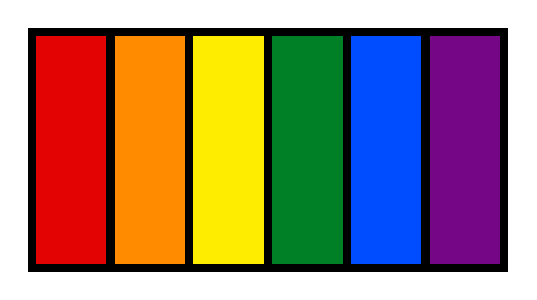
\begin{tikzpicture}[line width=3pt, baseline=0.75cm]
	\filldraw[fill=prideRed]    (0,0) rectangle (1,3);
	\filldraw[fill=prideOrange] (1,0) rectangle (2,3);
	\filldraw[fill=prideYellow] (2,0) rectangle (3,3);
	\filldraw[fill=prideGreen]  (3,0) rectangle (4,3);
	\filldraw[fill=prideBlue]   (4,0) rectangle (5,3);
	\filldraw[fill=pridePurple] (5,0) rectangle (6,3);
\end{tikzpicture}$
+
$
\begin{tikzpicture}[line width=3pt, baseline=0.75cm]
	\filldraw[fill=black] (0,0) rectangle (3,3);
	\filldraw[fill=white] (3,0) rectangle (6,3);
\end{tikzpicture}$
אל מול
$
\begin{tikzpicture}[line width=3pt, baseline=0.75cm]
	\filldraw[fill=IOF] (0,0) rectangle (6,3);
\end{tikzpicture}$
+
$
\begin{tikzpicture}[line width=3pt, baseline=0.75cm]
	\filldraw[fill=txelet] (0,0) rectangle (3,3);
	\filldraw[fill=white]  (3,0) rectangle (6,3);
\end{tikzpicture}$

\vfill

~

\end{center}


\newpage

\begin{center}

\changesize{120}
המיליטריזם והלאומנות
\end{center}

\vfill

\changesize{75}\fontspec{Guttman Haim-Condensed}

\hspace{4cm}
\begin{minipage}{0.8\linewidth}
\begin{itemize}
	\itemsep2cm
		\renewcommand{\labelitemi}{\LR{\altsymbolglyph{~☠}}}
	\item מגואלים בדם\\
		\renewcommand{\labelitemi}{\LR{\symbolglyph{~💪}}}
	\item משחיתים את החברה והיחיד\\
		\renewcommand{\labelitemi}{\LR{\symbolglyph{~👹}}}
	\item {\changesize{75}\fontspec{Guttman Haim-Condensed}מבוססים על שנאה, אלימות ואי־צדק}
		\renewcommand{\labelitemi}{\LR{\symbolglyph{~💰}}}
	\item {\changesize{75}\fontspec{Guttman Haim-Condensed}מהווים מעמסה מיותרת ומזיקה}
\end{itemize}
\end{minipage}

\vfill

~

\vfill

~


\end{document}
